\documentclass{article}
\usepackage{setspace}
\usepackage{geometry}
\usepackage[utf8]{inputenc}
\usepackage{amsmath,amsthm,amssymb,bm}
\usepackage{mathtools}

\geometry{letterpaper, portrait, margin=1in}
\setstretch{1.5}
\title{Homework 7}
%\date{1-18-2020}
\author{Runmin Lu}

\begin{document}
	\maketitle
	%\newpage
	
	\section*{1}
		Classification Algorithm: Linear Regression for classification followed by pocket for improvement.
		\subsection*{(a)}
			Training:\\
			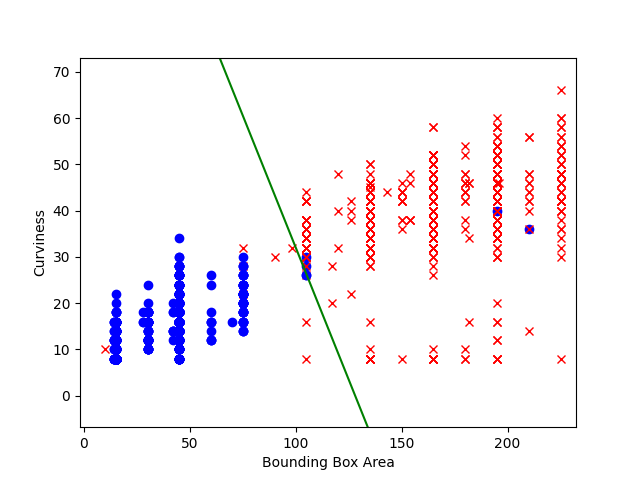
\includegraphics[scale=0.5]{train.png}\\
			Testing:\\
			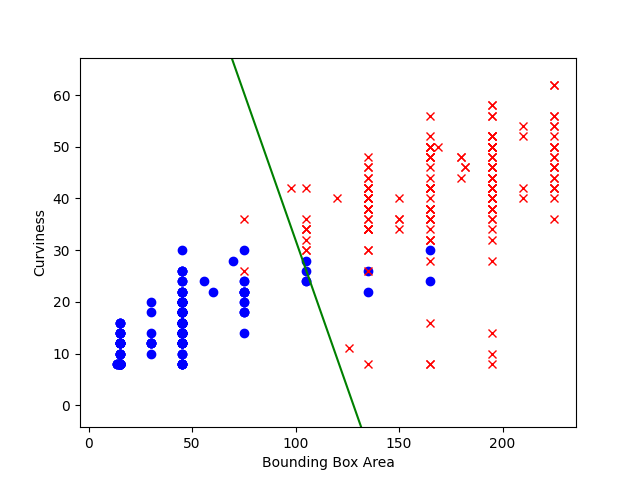
\includegraphics[scale=0.5]{test.png}
	
		\subsection*{(b)}
			\begin{align*}
				E_{\text{in}} &\approx 0.00833\\
				E_{\text{test}} &\approx 0.0165
			\end{align*}
	
		\subsection*{(c)}
			From $E_{\text{in}}$:
			\begin{align*}
				E_{\text{out}} &\leq E_{\text{in}} + \sqrt{ \frac8N \ln \frac{4(2N)^3}\delta }\\
				&\approx 0.00833 + \sqrt{ \frac8{1561} \ln \frac{4(2\times 1561)^3}{0.05} }\\
				&\approx 0.00833 + 0.3823\\
				&= \boxed{0.3906}
			\end{align*}
			From $E_{\text{test}}$:
			\begin{align*}
				E_{\text{out}} &\leq E_{\text{test}} + \sqrt{ \frac1{2K} \ln \frac{2}\delta }\\
				&\approx 0.0165 + \sqrt{ \frac1{424} \ln \frac{2}{0.05} }\\
				&\approx 0.0165 + 0.0933\\
				&= \boxed{0.1098} \leftarrow \text{The Better Bound}
			\end{align*}
			
		\subsection*{(d)}
			Training:\\
			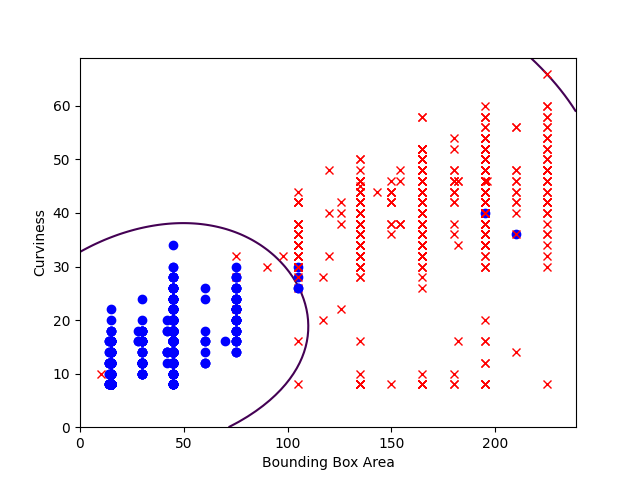
\includegraphics[scale=0.5]{train_3o.png}
			\begin{align*}
				E_{\text{in}} &\approx 0.00769\\
				E_{\text{out}} &\leq E_{\text{in}} + \sqrt{ \frac8N \ln \frac{4(2N)^{10}}\delta }\\
				&\approx 0.00769 + \sqrt{ \frac8{1561} \ln \frac{4(2\times 1561)^{10}}{0.05} }\\
				&\approx 0.00833 + 0.6589\\
				&= \boxed{0.6671}
			\end{align*}
			Testing: 
			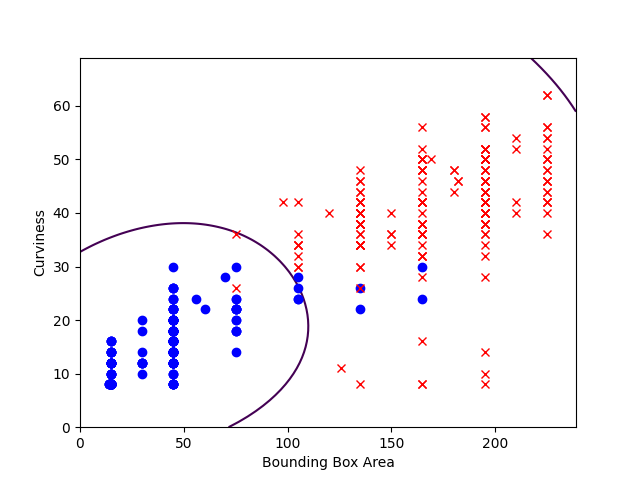
\includegraphics[scale=0.5]{test_3o.png}
			\begin{align*}
				E_{\text{test}} &\approx 0.0165\\
				E_{\text{out}} &\leq E_{\text{test}} + \sqrt{ \frac1{2K} \ln \frac{2}\delta }\\
				&\approx 0.0165 + \sqrt{ \frac1{424} \ln \frac{2}{0.05} }\\
				&\approx 0.0165 + 0.0933\\
				&= \boxed{0.1098} \leftarrow \text{The Better Bound}
			\end{align*}
			
		\subsection*{(e)}
			I would use the linear model because even though both models produce similar $E_{\text{test}}$, the visualization of the third order model just does not make sense with the boundary at the upper right corner. There's no way that a digit with even bigger bounding box and more curve is more likely to be a 1.
			
	\section*{2}
	\subsection*{(a)}
		\begin{align*}
			\nabla f(x, y) =
			\begin{pmatrix}
				2x + 4\pi \cos (2\pi x)\sin (2\pi y)\\
				4y + 4\pi \sin (2\pi x)\cos (2\pi y)
			\end{pmatrix}
		\end{align*}
		For $\eta = 0.01$:\\
		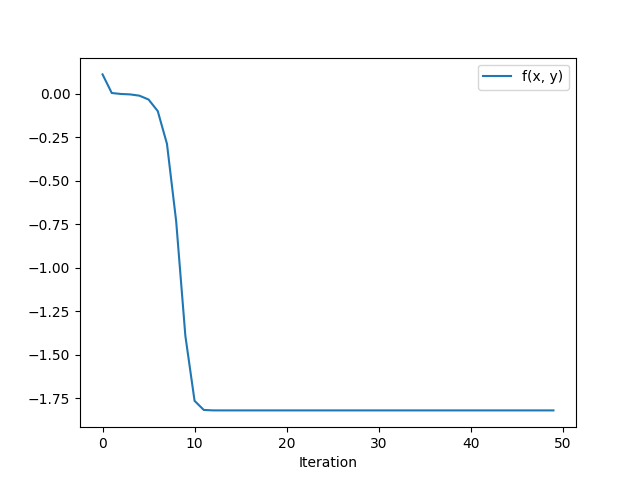
\includegraphics[scale=0.7]{2a1.png}\\
		For $\eta = 0.1$:\\
		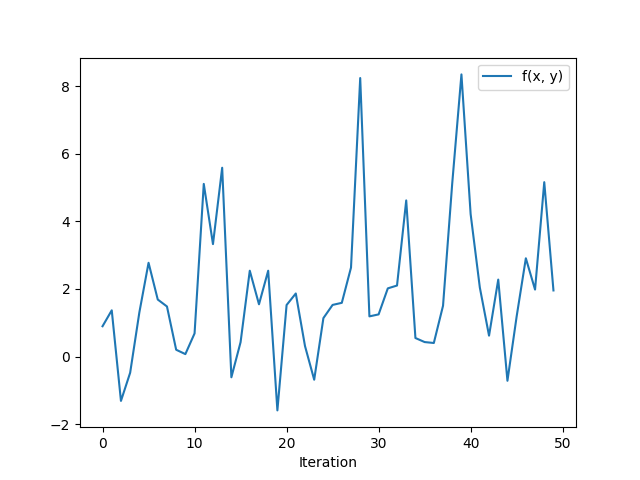
\includegraphics[scale=0.7]{2a2.png}\\
		$f(x, y)$ changes unpredictably because the step is too large. $(x, y)$ in each step sometimes moves to the other side of the local minimum, which potentially increases $f(x, y)$.
		
	\subsection*{(b)}
		\begin{tabular}{c|cccc}
			initial point & (0.1, 0.1) & (1, 1) & (-0.5, -0.5) & (-1, -1)\\
			\hline
			argmin $f(x, y)$ & (0.244, -0.238) & (1.218, 0.713) & (-0.731, -0.238) & (-1.218, -0.713)\\
			\hline
			$\min f(x, y)$ & -1.820 & 0.593 & -1.332 & 0.593
		\end{tabular}
		
	\section*{Problem 3.16}
	\subsection*{(a)}
		\begin{align*}
			\text{cost}(\text{accept}) &= P[\text{correct}]\times 0 + P[\text{incorrect}]c_a\\
			&= P[\text{incorrect}]c_a\\
			&= (1-g(\mathbf x))c_a\ \ \ \ \ \ \text{because } g(\mathbf x) \text{ is the probablilty that this person is correct}\\
			\text{cost}(\text{reject}) &= P[\text{correct}]c_r + P[\text{incorrect}] \times 0\\
			&= P[\text{correct}]c_r\\
			&= g(\mathbf x)c_r
		\end{align*}
	\subsection*{(b)}
		\begin{align*}
			\text{Let }C &= \text{ the total cost of actions taken on each person}\\
			&= \sum\limits_{\mathbf x: g(\mathbf x) \geq \kappa}\text{cost}(\text{accept}) + \sum\limits_{\mathbf x: g(\mathbf x) < \kappa}\text{cost}(\text{reject})\\
			&= \sum\limits_{\mathbf x: g(\mathbf x) \geq \kappa}(1-g(\mathbf x))c_a + \sum\limits_{\mathbf x: g(\mathbf x) < \kappa}g(\mathbf x)c_r\\
		\end{align*}
		Consider $\frac{dC}{d\kappa}$ as the change in $C$ if we increase $\kappa$ a little bit such a single accepted data point $\mathbf x^*$ is now rejected. we know that $g(\mathbf x^*) = \kappa$.\\
		To minimize $C$ with respect to $\kappa$, we set $\frac{dC}{d\kappa}$ to 0.
		\begin{align*}
			\frac{dC}{d\kappa} &= -(1-g(\mathbf x^*))c_a + g(\mathbf x^*)c_r\\
			&= -(1-\kappa)c_a + \kappa c_r\\
			&= \kappa(c_a + c_r) - c_a\\
			&= 0\\
			\kappa &= \frac{c_a}{c_r + c_a}					
		\end{align*}
	
	\subsection*{(c)}
		Supermarket: $\kappa = \frac1{11}$\\
		Because it costs a lot to reject someone, we want to accept as many as possible, which results in a lower $\kappa$.\\
		CIA: $\kappa = \frac{1000}{1001}$\\
		Because it costs a lot to accept someone, we want to reject as many as possible, which results in a higher $\kappa$. 
\end{document}